\documentclass{beamer}

\usetheme{Madrid}
\usepackage[utf8]{inputenc}
\usepackage[T1]{fontenc}
\usepackage{graphicx}
\usepackage{booktabs}
\usepackage{amsmath}
\usepackage{placeins}

\graphicspath{{./}{../../assets/}{../../outputs/}{../../docs/images/}}

\title[Road Segmentation]{Road Segmentation from Satellite Imagery}
\subtitle{A Comparison of Deep Learning and Traditional Baselines}
\author[Wayn, Xavier]{William Wayn \and Maysa Xavier}
\institute[UWS]{%
  COMP11069 -- Data Mining and Visualisation \\
  University of the West of Scotland%
}
\date{2025/2026}

% ---------------------
\begin{document}

\begin{frame}
  \titlepage
\end{frame}

\begin{frame}{Outline}
  \tableofcontents
\end{frame}

% =====================
\section{The Problem}

\begin{frame}{The Problem}
  \begin{columns}[T]
    \column{0.55\textwidth}
    \begin{block}{The intuition}
      Imagine holding a satellite photograph and being asked to draw every road.
      Your eye finds them immediately: thin grey threads snaking through fields.
      Your brain reads \textit{context}.
    \end{block}
    \vspace{0.5em}
    A computer sees only numbers.
    The grey of asphalt in full sun is nearly identical to dry riverbed in shadow.

    \vspace{0.5em}
    \textbf{The signal is spatial, not spectral.}

    \column{0.45\textwidth}
    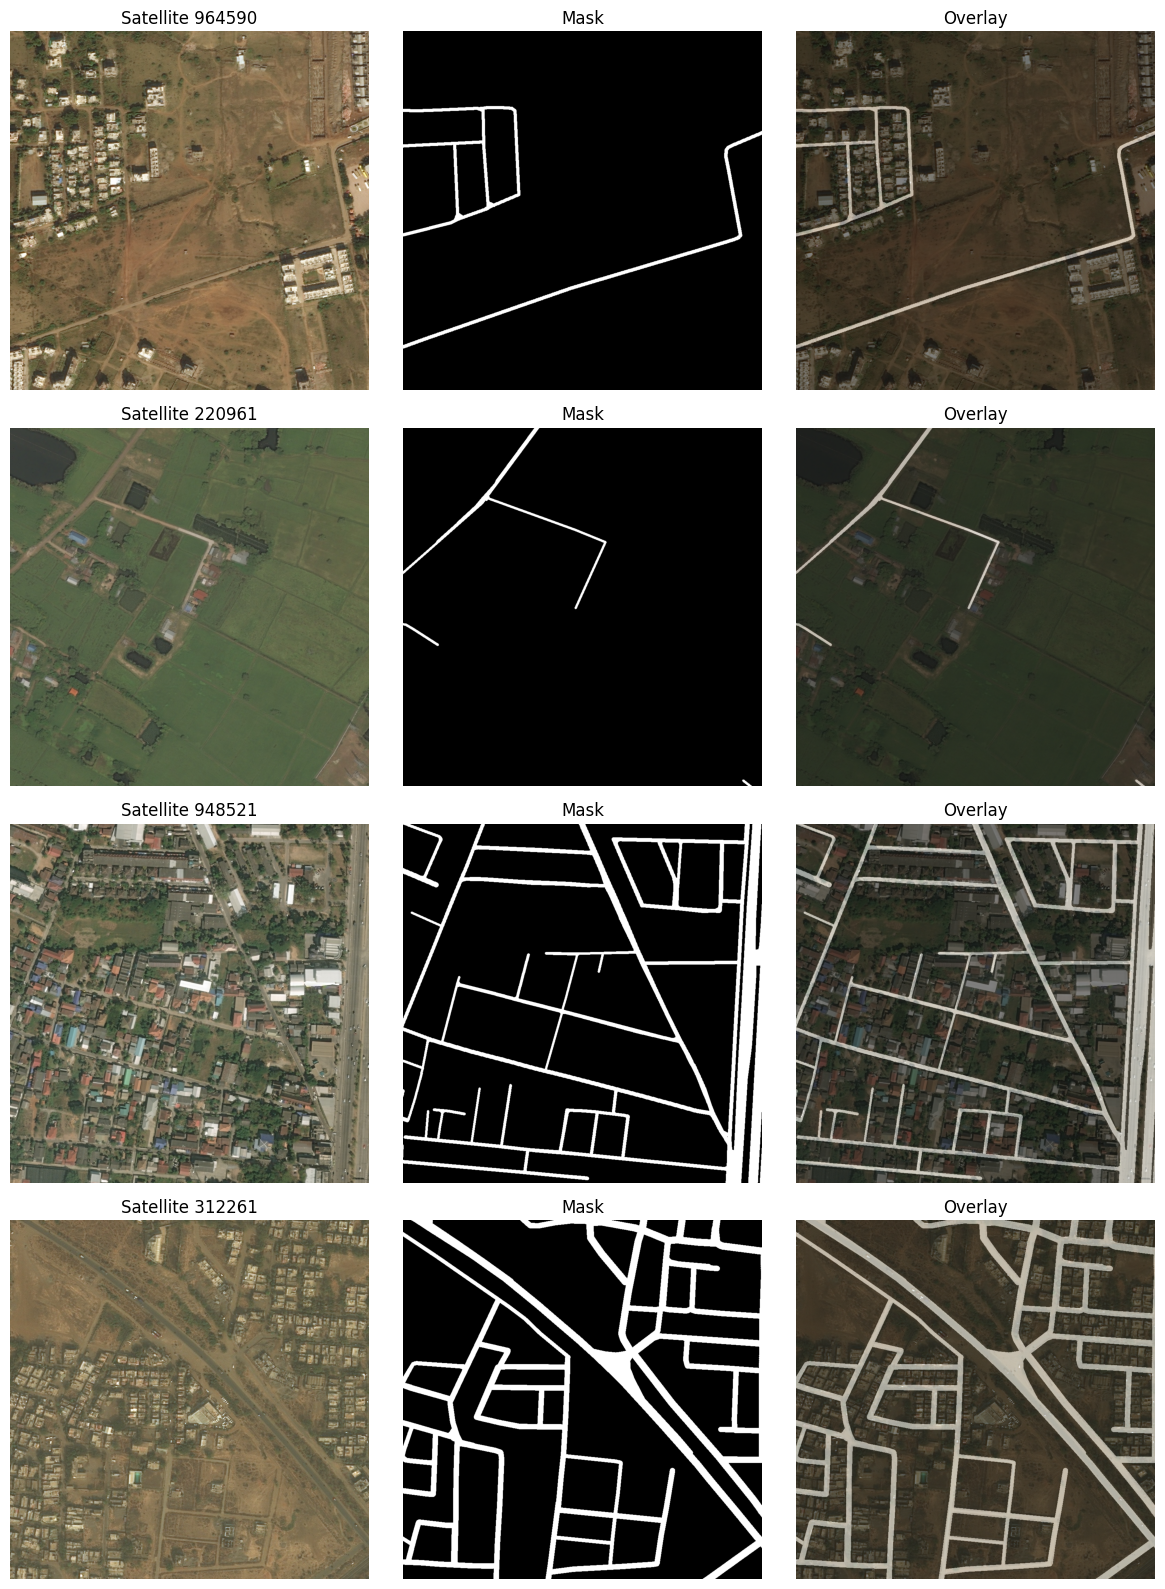
\includegraphics[width=\linewidth]{images_example.png}
  \end{columns}
\end{frame}

% =====================
\section{Dataset \& EDA}

\begin{frame}{DeepGlobe Road Extraction}
  \begin{columns}[T]
    \column{0.55\textwidth}
    \begin{itemize}
      \item $1024\times1024$ px, 50\,cm/pixel GSD
      \item Thailand, Indonesia, India
      \item \textbf{803} train / \textbf{171} val / 172 test
      \item Resized to $256\times256$ for training \\
            (trade-off discussed in limitations)
    \end{itemize}
    \vspace{0.5em}
    The dataset spans wide urban arteries to thin dirt tracks, presenting a broad range of difficulty.

    \column{0.45\textwidth}
    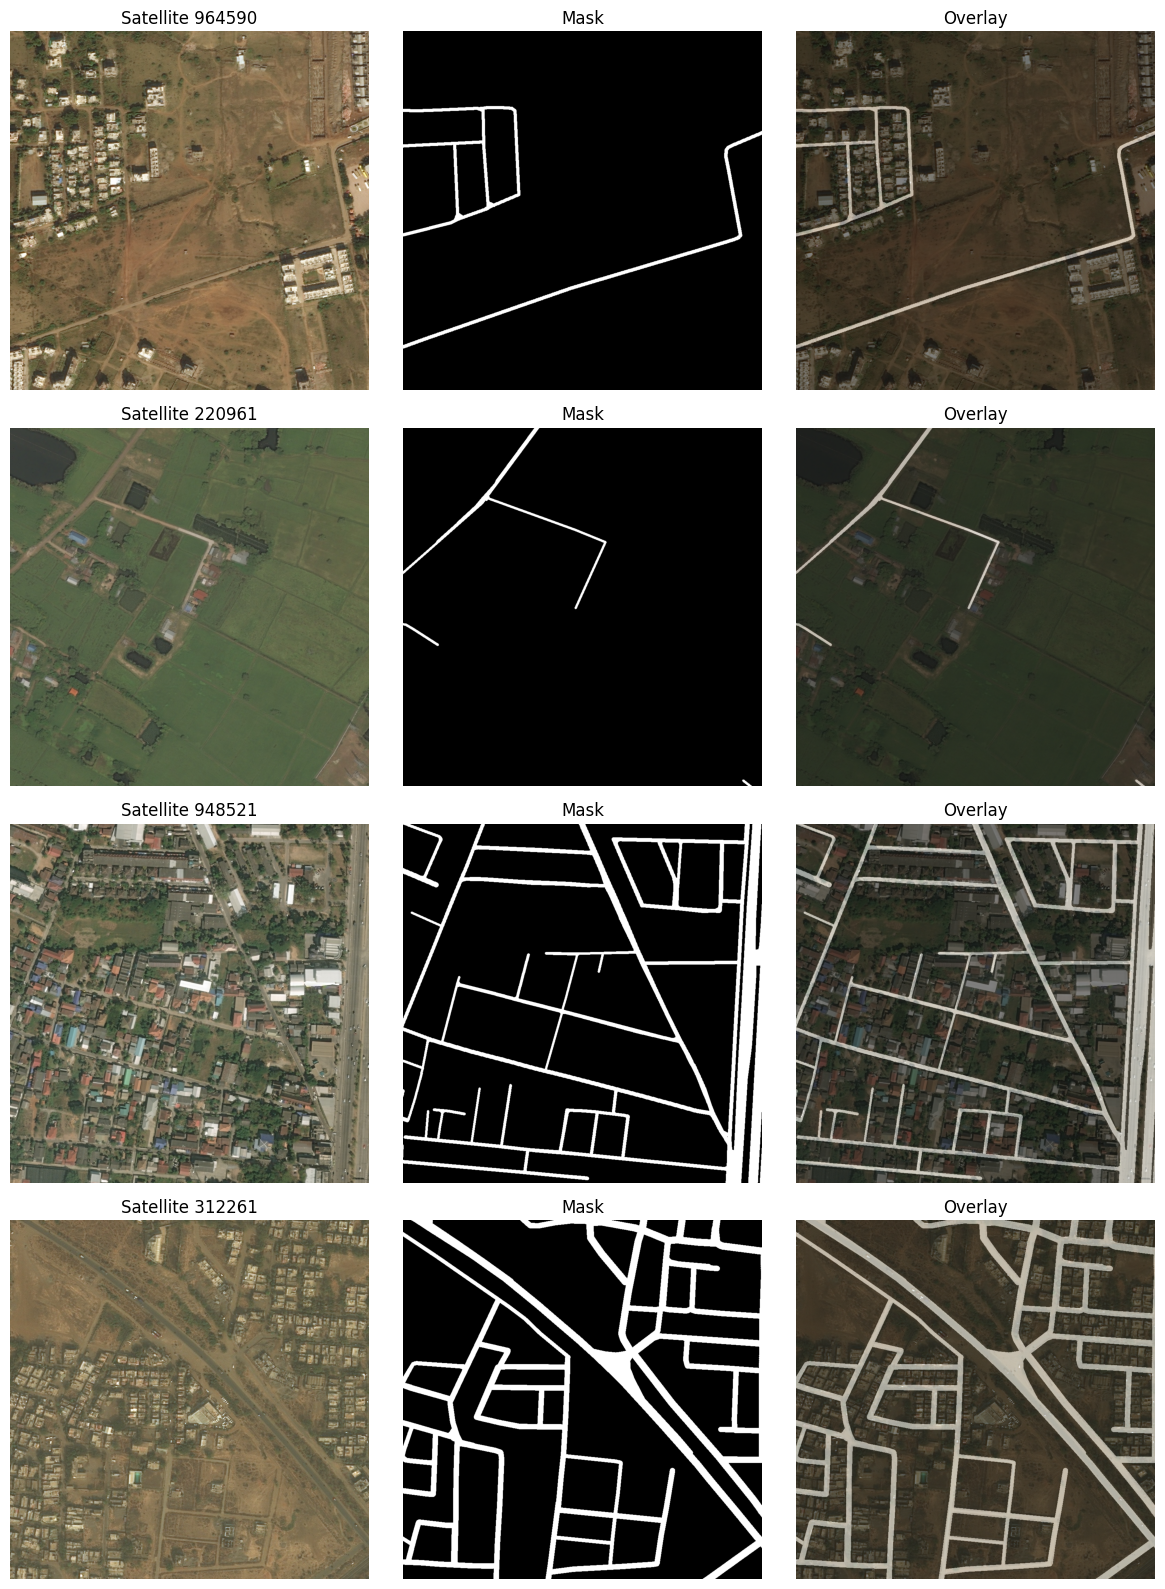
\includegraphics[width=\linewidth]{images_example.png}
  \end{columns}
\end{frame}

\begin{frame}{Two Challenges That Drive Everything}
  \begin{enumerate}
    \item \textbf{Class imbalance}
    \begin{itemize}
      \item Roads cover only 4--8\% of each tile
      \item Predicting ``no road'' everywhere $\Rightarrow$ $>$92\% pixel accuracy
      \item[$\Rightarrow$] We use \textbf{IoU}, not accuracy
    \end{itemize}
    \vspace{0.8em}
    \item \textbf{Thin, elongated structures}
    \begin{itemize}
      \item Each pixel is equivalent to roughly half a metre on the ground
      \item After resizing to $256\times256$, rural roads are 3--5 pixels wide
      \item A model that discards spatial resolution cannot recover them
      \item[$\Rightarrow$] Architecture must \textit{preserve} spatial detail
    \end{itemize}
  \end{enumerate}
  \vspace{0.2em}
  
  \begin{columns}[c]
    \column{0.4\textwidth}
    \centering
    \small\textit{Metric: Intersection over Union}
    \begin{equation*}
      \text{IoU} = \frac{|\hat{Y} \cap Y|}{|\hat{Y} \cup Y|}
    \end{equation*}

    \column{0.6\textwidth}
    \centering
    
\includegraphics[width=\linewidth,height=0.25\textheight,keepaspectratio]{iou_diagram.pdf}
  \end{columns}

  \vspace{0.3em}
  \centering
  \small\textit{These two observations will govern every choice we make.}
\end{frame}

% =====================
\section{Methods}

\begin{frame}{Our Approach: A Ladder of Complexity}
  \begin{center}
    \begin{tabular}{clll}
      \toprule
      Rung & Method & What it adds \\
      \midrule
      1 & RGB Thresholding       & Colour statistics \\
      2 & K-Means Clustering     & Colour grouping \\
      3 & \textbf{U-Net}         & Spatial context + local detail \\
      \bottomrule
    \end{tabular}
  \end{center}
  \vspace{0.8em}
  \centering
  We start simple. We add complexity only when the data demands it.
\end{frame}

\begin{frame}{Rung 1: RGB Thresholding}
  \begin{columns}[c]
    \column{0.55\textwidth}
    \textbf{Global Colour Thresholds}
    \begin{itemize}
      \item \textbf{Method:} Analysed pixel colour distributions to find optimal separation thresholds.
      \item \textbf{Evaluation:} Tested 5 channels (RGB, Grayscale, Luminance), selecting the one yielding the highest IoU.
      \item \textbf{Result:} Performs poorly, as predicted by our EDA.
    \end{itemize}
    \vspace{0.8em}
    \textbf{The Fundamental Flaw:} \\
    Colour statistics alone cannot distinguish sunlit asphalt from a white roof, or shaded roads from a riverbed.

    \column{0.45\textwidth}
    \centering
    \includegraphics[width=\linewidth,height=0.85\textheight,keepaspectratio]{baselines/rgb_threshold_cropped.png}
    \end{columns}
  \end{frame}

\FloatBarrier

\begin{frame}{Rung 2: K-Means Clustering}
  \begin{columns}[c]
    \column{0.55\textwidth}
    \textbf{K-Means Clustering} ($k=2$)
    \begin{itemize}
      \item \textbf{Method:} Algorithm finds colour clusters without supervision.
      \item \textbf{Evaluation:} Clusters are labelled road/non-road based on overlap with ground-truth masks.
      \item \textbf{Result:} Marginally better than single thresholds, but still strictly pixel-level with no spatial context.
    \end{itemize}
    \vspace{0.8em}
    \textbf{The Fundamental Flaw:} \\
    Grouping pixels into colour clusters provides cleaner boundaries, but still inherently fails to capture the thread-like extended shapes of roads.

    \column{0.45\textwidth}
    \centering
    \includegraphics[width=\linewidth,height=0.85\textheight,keepaspectratio]{baselines/kmeans_cropped.png}
    \end{columns}
  \end{frame}

\FloatBarrier

\begin{frame}{Rung 3: U-Net}
  \begin{columns}[T]
    \column{0.55\textwidth}
    Proposed by Ronneberger, Fischer \& Brox (2015) for biomedical segmentation. \\
    The defining feature: \textbf{skip connections}. \\
    Encoder features concatenate directly into the matching decoder. \\
    \begin{itemize}
      \item High-resolution detail is \textit{preserved}, not reconstructed
      \item Exactly what the thin-road observation demanded
      \item 31.0\,M parameters, trained from scratch
      \item Augmentation pipeline improves generalisation
      \item 30 epochs, Adam $\eta=10^{-4}$, BCE loss
    \end{itemize}

    \column{0.45\textwidth}
    \includegraphics[width=\linewidth]{unet/training_curves.png}
    \vspace{0.2em}
    \small\centering
    Clean convergence: val.\ loss tracks training throughout.
  \end{columns}
\end{frame}

\begin{frame}[shrink=8]{U-Net: Training Augmentation}
  \begin{columns}[T]
    \column{0.38\textwidth}
    \small
    \textbf{Why we used it}
    \begin{itemize}
      \item Only \textbf{803} training images
      \item Clear risk of overfitting to fixed orientations and layouts
      \item Roads should remain roads after flips, rotations, and small affine shifts
    \end{itemize}
    \vspace{0.3em}
    \textbf{Pipeline}
    \begin{itemize}
      \item Horizontal and vertical flips
      \item Random 90/180/270-degree rotations
      \item Small affine rotation, translation, and scale jitter
      \item \textbf{Important:} image and mask are transformed together
    \end{itemize}

    \column{0.62\textwidth}
    \centering
    \includegraphics[width=\linewidth,height=0.56\textheight,keepaspectratio]{augmentation_preview/augment_overlay_4_presentation_2x2_948521.png}
  \end{columns}
\end{frame}

\begin{frame}{The U-Net Architecture}
  \begin{columns}[c]
    \column{0.45\textwidth}
    \textbf{Encoder} (Contracting Path)
    \begin{itemize}
      \item Extracts semantic context
      \item Gradually reduces spatial dimensions
    \end{itemize}
    \vspace{0.8em}
    \textbf{Decoder} (Expansive Path)
    \begin{itemize}
      \item Upsamples back to original resolution
      \item \textbf{Skip connections:} transfer high-resolution features directly from the encoder
    \end{itemize}
    \vspace{0.8em}
    \textit{This bypasses the compression bottleneck, making it ideal for thin, elongated road structures.}

    \column{0.55\textwidth}
    \centering
    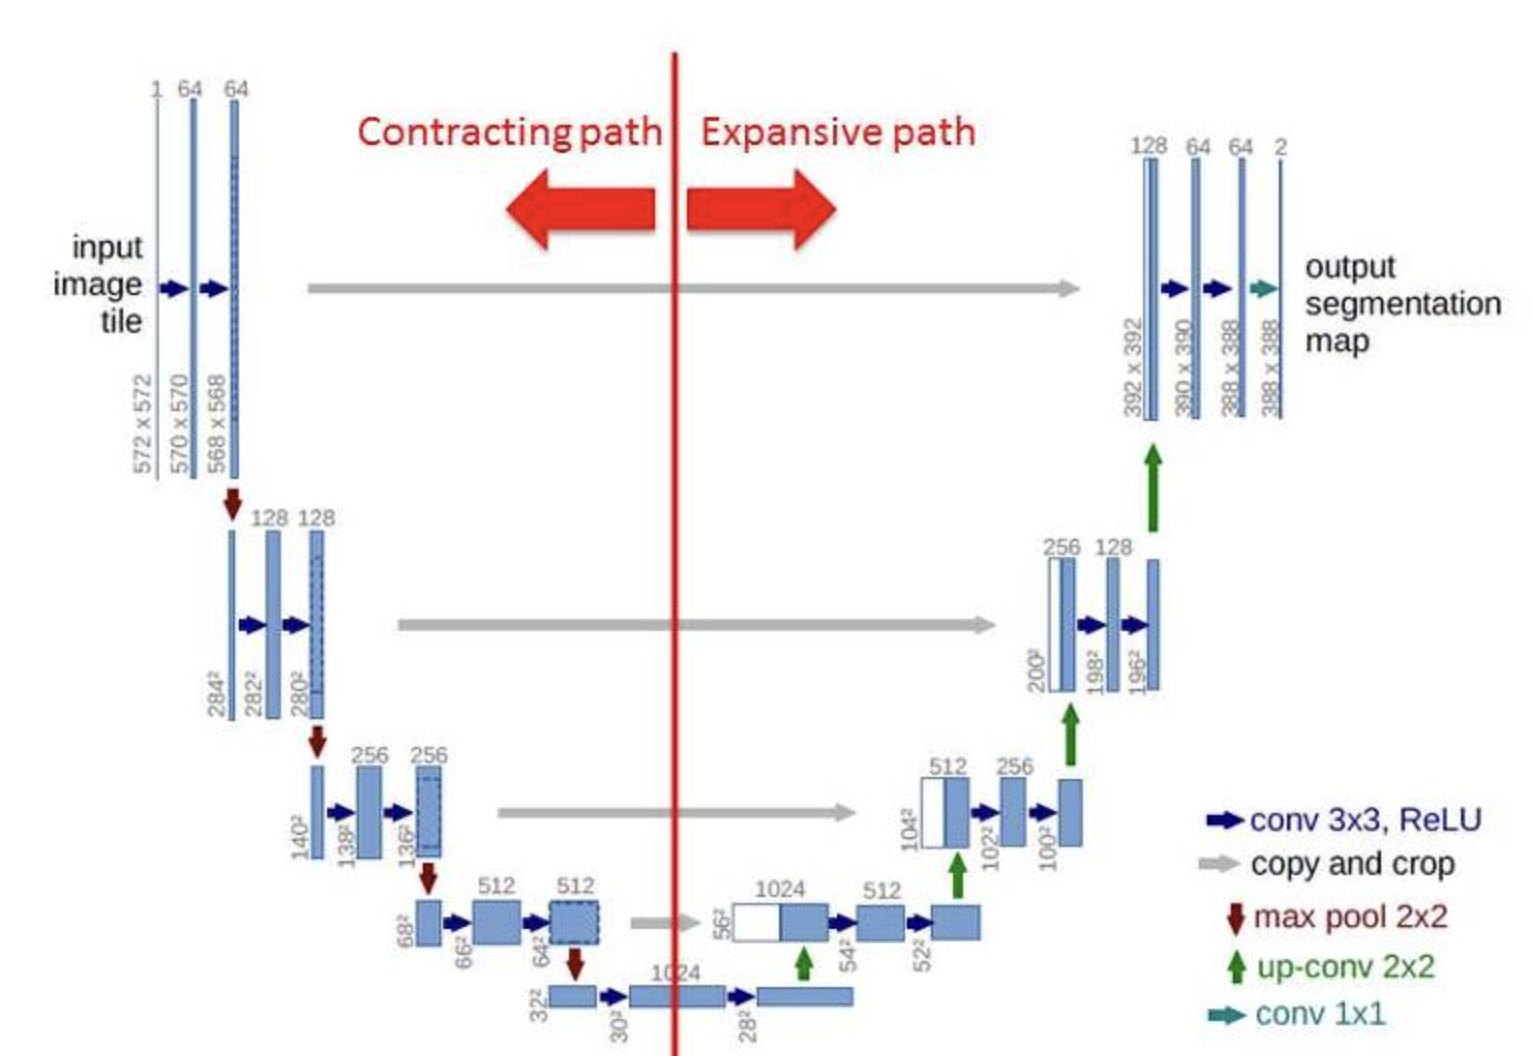
\includegraphics[width=\linewidth,height=0.7\textheight,keepaspectratio]{UNetArchitecture.png}
  \end{columns}
\end{frame}

% =====================
\section{Results}

\begin{frame}{Results: Quantitative}
  \begin{center}
    \begin{tabular}{lcc}
      \toprule
      Method                  & Val.\ IoU        & Parameters \\
      \midrule
      RGB Thresholding (KS)   & $\sim$0.15--0.25 & -- \\
      K-Means ($k=2$)         & $\sim$0.20--0.30 & -- \\
      U-Net ($512\times512$)  & 0.565            & 31.0\,M \\
      \textbf{U-Net ($256\times256$)} & \textbf{0.588}   & 31.0\,M \\
      \bottomrule
    \end{tabular}
  \end{center}
  \vspace{0.5em}
  U-Net outperforms the classical baselines by over \textbf{0.30 IoU points}.
\end{frame}

% =====================
\section{Discussion}

\begin{frame}{The Resolution Paradox: $256\times256$ vs $512\times512$}
  We experimented with higher resolution ($512\times512$) to better preserve thin roads.
  \vspace{0.5em}
  
  \begin{block}{The Paradox}
    \begin{itemize}
      \item \textbf{$256\times256$ (IoU 0.588):} Downsampling heavily blurs thin roads, artificially thickening them. The model overlaps these inflated areas more easily, resulting in higher mathematical IoU.
      \item \textbf{$512\times512$ (IoU 0.565):} Higher resolution keeps roads thinner and more accurate to reality. However, IoU heavily penalises slight 1-pixel misalignments at the boundaries.
    \end{itemize}
  \end{block}
  \vspace{0.5em}
  \textbf{Takeaway:} The higher resolution model preserves the true topology of the road network better qualitatively, even if strict exact-pixel IoU matching decreases.
\end{frame}

\section{Conclusion}

\begin{frame}{Limitations and The Main Lesson}
  \begin{columns}[T]
    \column{0.4\textwidth}
    \textbf{Honest limitations}
    \begin{itemize}
      \item One geographic region only (South \& SE Asia)
      \item No evidence of generalisation to other sensors or seasons
    \end{itemize}

    \column{0.6\textwidth}
    \textbf{The main lesson}
    \begin{itemize}
      \item Reading the data carefully mattered more than defaulting to the biggest model
      \item Thin, sparse, spectrally heterogeneous roads pointed us to U-Net before training
      \item The results confirmed that intuition: \textbf{U-Net 0.588} vs. baselines $\leq$ 0.30
      \item Inductive bias matters when the task has a clear structural requirement
    \end{itemize}
  \end{columns}
  \vspace{0.5em}
  \centering
  \textit{Thank you.}
\end{frame}

\end{document}
